%-------------------------------------------------------------------------------
% RESULTS
%-------------------------------------------------------------------------------

\section{Results \red{and Discussion}} \label{sec:res}

\subsection{Outline of Bifurcation Diagram}

The primary objective of this project is to reproduce and complete the
bifurcation diagram presented in figure \ref{fig:bif_diag_chen} of
\citet{chen2013}. The resulting bifurcation diagram of the regularized version
is depicted in figure \ref{fig:bif_diag}, and table \ref{tab:bif_points} lists
the bifurcations that occurre along with their corresponding critical Reynolds
numbers. Table \ref{tab:re_crit} shows the critical Reynolds numbers obtained
for different grid sizes. As mentioned, only a square cavity is considered for
this study, and no aspect ratios have been varied.

The critical Reynolds numbers reported here are determined by interpolating the
leading eigenvalues between states of the pseudo-arclength continuation
algorithm where the leading eigenvalue crosses the imaginary axis in the
complex plane. The reported results are rounded to three significant digits.

\begin{table}[h!]
  \centering
  \caption{List of bifurcations encountered and the critical $\Rey$ at which they
    occur}
  \label{tab:bif_points}
\begin{tabular}{l c}
Bifurcation & $\Rey$\\
\hline
$P_1$, first supercritical pitchfork of the base flow & $66.197$ \\
$P_2$, second pitchfork of the base flow & $172.708$ \\
$P_3$, pitchfork of the asymmetric steady solution & $353.357$ \\
$SN$, saddle-node bifurcation of the asymmetric steady solution & $353.654$ \\
$H$, Hopf bifurcation of the asymmetric steady solution & $348.319$ \\
\end{tabular}
\end{table}

\begin{table}[h!]
  \centering
  \caption{Critical Reynolds numbers for different grid sizes $m$ of the two
    pitchfork bifurcations of the symmetric base flow, $\Rey_c^{P_1}$ and
    $\Rey_c^{P_2}$, and of the saddle-node, the third pitchfork, and Hopf
    bifurcations corresponding to the asymmetric steady solution,
    $\Rey_c^{SN}$, $\Rey_c^{P_3}$ and $\Rey_c^{H}$ respectively. For the Hopf
    bifurcation, the imaginary part $\omega_c^{H}$ corresponding to the
    crossing eigenvalue has also been included. In comparison, the scaled
    critical values for the un-regularized version are shown as well.}
  \label{tab:re_crit}
\begin{tabular}{crrrrrr}
$m$ & $\Rey_c^{P_1}$ & $\Rey_c^{P_2}$ & $\Rey_c^{H}$ &  $\omega_c^{H}$ & $\Rey_c^{P_3}$ & $\Rey_c^{SN}$  \\
\hline
$32$ & $66.197$ & $172.731$ & $348.210$ & $0.0582$ & $352.152$ & $352.527$ \\
$48$ & $66.197$ & $172.708$ & $348.312$ & $0.0588$ & $353.365$ & $353.663$ \\
$64$ & $66.197$ & $172.708$ & $348.319$ & $0.0599$ & $353.356$ & $353.656$ \\
$96$ & $66.197$ & $172.708$ & $348.319$ & $0.0599$ & \red{$353.357$} & $353.654$ \\
\citet{chen2013} & $65.154$ & $177.723$ & - $\quad$ & - $\quad$ & - $\quad$ & $438.285$ \\
\end{tabular}
\end{table}

\begin{figure}[!htb]
  \begin{tikzpicture}
    \node[anchor=south west,inner sep=0] (image) at (0,0) {\includegraphics[width=0.9\textwidth]{figs/bifurcation_diag64x64.pdf}};
      \begin{scope}[x={(image.south east)},y={(image.north west)}]
          \draw (0.872,0.72) circle [radius=14pt];
          \draw[-latex] (0.92,0.728) -- (0.95,0.733);
          \node[anchor=south west,inner sep=0] (image) at (0.8,0.65) {\includegraphics[width=0.3\textwidth]{figs/bifurcation_diag_zoom64x64.pdf}};
      \end{scope}
  \end{tikzpicture}
  \caption{Bifurcation diagram for the regularized version of the four-sided
    cavity flow, calculated by using the custom-developed Julia module} 
  \label{fig:bif_diag}
\end{figure}

Analyzing the new bifurcation diagram in figure \ref{fig:bif_diag} shows that
the regularized version resembles the non-regularized one regarding
bifurcations and the shape of the asymmetric branches. The reported critical
Reynolds numbers for the pitchforks $P_1$ and $P_2$ are close to those of the
original problem (a factor of $2$, with respect to Chen's scaling, see section
\ref{sec:regul}). We can also see how the regularized version converges
rapidly, with only changes within the third decimal digit (or smaller) for a grid
of size $48 \times 48$ or larger for the two pitchforks and the saddle-node
bifurcation.

On the other hand, it has been observed that the critical value for the
saddle-node in the regularized version deviates significantly from the original
value by approximately $80$ units of Reynolds. This variation is probably
caused by the regularization. However, measuring the discrepancy as a function
of the control parameter $k_0$ is out of the scope of this work.

Moreover, the Group of Nonlinear Fluid Dynamics at UPC has recently discovered
a Hopf bifurcation ($H$) at the asymmetric branch. Furthermore, a pitchfork
bifurcation ($P_3$) has also been found with a critical Reynolds number close
to the saddle-node. Another branch is emerging at that location, displaying a
different asymmetric flow pattern. The following two subsections will discuss
these two bifurcation scenarios in more detail.

\subsection{Hopf Bifurcation and Time-Periodic Flows}

The Hopf bifurcation is found to be located at a critical Reynolds of $348.319$
and has not been reported in previous studies to our knowledge. The question
that arises is whether the Hopf bifurcation is subcritical or
supercritical. 

Figure \ref{fig:hopf} in section \ref{sec:bif_details} on bifurcation scenarios
shows how these two types differ. For a supercritical Hopf, we would expect
stable periodic orbits for a Reynolds number above the critical value of the
Hopf bifurcation. On the contrary, for the subcritical case, unstable periodic
orbits should be located below the critical value. The amplitudes of the
periodic orbits, for both cases, should scale following a square root envelope
of the form, $A \propto \lvert R - R_c \rvert^{\frac{1}{2}}$
\citep{kuznetsov2004}. 

To investigate the above, the time-stepper is launched from the perturbed
symmetric unstable solution at Reynolds number larger than the critical value
of the Hopf. These time evolutions reveal trajectories that converge to stable
periodic orbits (see figure \ref{fig:orbits}), but the amplitudes of these
oscillations are larger than the expected square root growth for a
supercritical Hopf. Further, the Group of Nonlinear Fluid Dynamics has computed
unstable periodic orbits that converge subcritically from the Hopf bifurcation
at $\Rey = \Rey_c^H$. At smaller Reynolds numbers, the unstable periodic orbits
collapse in a homoclinic connection with the lower asymmetric branch. These
results confirm that the Hopf is subcritical.

The follow-up questions revolve around the detected stable periodic orbits with large
amplitudes. They are depicted in figure \ref{fig:orbits} for three distinct
Reynolds numbers. The orbits are visualized in a projection of the phase space
using the average of the vertical and horizontal velocities at the top and left
mid-points of the cavity (as defined in figure \ref{fig:cav_domain}). In figure
\ref{fig:orbits}, the amplitudes of these oscillations are also shown by
extracting the center value of the streamfunction. They are compared to the
steady-state branches in the bifurcation diagram. 

Moreover, as shown in the figure, these stable periodic orbits with large
amplitude exist below the Hopf bifurcation's critical value and were obtained
by extracting the solutions of the matrix $\Psi$ with the maximum amplitude
from an orbit at a higher Reynolds number, and then this solution is used as an
initial condition for the time-stepper. In this way, one can "continue" stable
periodic orbits backward in Reynolds, similar to a natural continuation
algorithm. These periodic orbits collapse at a Reynolds number of around $335$,
and time evolutions at lower values will converge to one of the stable
asymmetric branches.

Figure \ref{fig:orbits_zoom} shows a zoom of the phase portrait of figure
\ref{fig:orbits} on the trajectories of the stable periodic orbits. The blue
dots refer to the values of the stationary solutions. One can recognize that
the stable periodic orbits transiently visit the locally attracting lower
saddle steady-state (LB), and the periodic orbit with a Reynolds number of
$336$ is approaching this fixed point even more (see figure
\ref{fig:orbits_zoom}). This suggests that the collapse at around $335$ in
Reynolds is through a heteroclinic connection with the unstable lower branches.

\begin{figure}[!h]
  \begin{subfigure}[b]{0.42\textwidth}
  \centering
  \includegraphics[trim={3cm 0 4.6cm 0},clip,width=\textwidth]{figs/orbits_bif_diag64x64.pdf}
  \end{subfigure}
  \begin{subfigure}[b]{0.58\textwidth}
  \centering
  \includegraphics[trim={1cm 0cm 1cm 0cm},clip,width=\textwidth]{figs/orbits64x64.pdf}
  \end{subfigure}
  \caption{Periodic orbits at different Reynolds numbers, amplitudes depicted
    in the bifurcation diagram and in a phase portrait using the velocities at
    the top and left mid-points of the cavity} 
  \label{fig:orbits}
\end{figure}

\begin{figure}[!htb]
  \begin{tikzpicture}
    \node[anchor=south west,inner sep=0] (image) at (0,0) {\includegraphics[trim={0 1cm 0 1cm},clip,width=0.8\textwidth]{figs/orbits_zoom64x64.pdf}};
    \node at (8, 4.5) {\small UB};
    \node at (11.1, 4.4) {\small LB};
  \end{tikzpicture}
  \caption{Zoom of periodic orbits at different Reynolds numbers, blue dots
    denote the locations of the upper stable (UB) and unstable (LB) steady
    solutions for $\Rey = 336$}
  \label{fig:orbits_zoom}
\end{figure}

It is unclear if the stable periodic orbits with a large amplitude below the
critical Reynolds number are related to the unstable periodic orbits of the
subcritical Hopf. Figure \ref{fig:sub_hopf_sketch} illustrates what seems to be
happening. One can see that there is an interval where two stable solutions
coexist, namely the stable asymmetric branch and the stable periodic orbits.
From a dynamical systems point of view, these stable solutions must be
separated by an unstable branch. 

An explanation, therefore, could be that the two periodic orbits are connected,
forming what is called a saddle-node of orbits. However, this does not seem to
be the case because the homoclinic connection and the collapse of the
subcritical periodic orbits take place at distinct Reynolds numbers. What the
separating branch is, remains unclear, but the Hopf bifurcation itself is
likely of subcritical type.

\begin{figure}[h!]
\centering
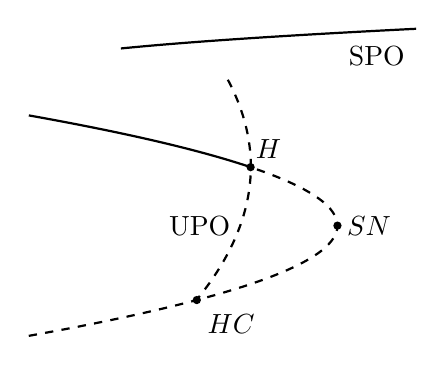
\begin{tikzpicture}[scale=0.5]
  \draw[thick, dashed] plot[smooth,domain=-2.8:1.5] ({-\x*\x},\x);
  \draw[thick] plot[smooth,domain=1.5:2.8] ({-\x*\x},\x);

  \draw[thick, dashed] plot[smooth,domain=-3.45:2.38] ({-0.12*\x*\x - 2.2},\x + 1.5);

  \draw[thick] plot[smooth,domain=0.5:1] ({10*\x*\x - 8},\x + 4);

  \fill (-1.485^2,1.485) circle [radius=3pt];
  \fill (-1.89^2,-1.89) circle [radius=3pt];
  \fill (0,0) circle [radius=3pt];

  \node at (-1.5^2 + 0.5,1.7 + 0.25) {$H$};
  \node at (-3.5,0) {UPO};
  \node at (1,4.3) {SPO};
  \node at (-2.7,-2.5) {$HC$};
  \node at (0.8,0) {$SN$};
\end{tikzpicture}
\caption{Illustration of amplitudes in the bifurcation diagram for the stable
  periodic (SPO) and the unstable periodic orbits (UPO) with its homoclinic
  connection ($HC$)} 
\label{fig:sub_hopf_sketch}
\end{figure}

\subsection{Pitchfork Bifurcation and New Asymmetric Solutions}

A linear stability analysis performed along the upper asymmetric branch has
also revealed that another real eigenvalue crosses the imaginary axis slightly
after the Hopf bifurcation and before reaching the saddle-node point. Figure
\ref{fig:lsa} shows the three rightmost eigenvalues in a plot where the
Reynolds number increases and then decreases again from the saddle-node
onwards. The details of these crossings are presented in table \ref{tab:cross}.
The crossing labeled $A$ corresponds to the complex conjugate pair associated
with the Hopf bifurcation, which is denoted by $\lambda_1$ and $\lambda_2$ in
green. However, another eigenvalue crossing is found just before the
saddle-node, denoted as $B$. This second eigenvalue crossing ($\lambda_3$ in
orange) lies within a range of $0.3$ in Reynolds. \\\\

\begin{minipage}[h]{\textwidth} \begin{minipage}[b]{.53\textwidth} \centering
  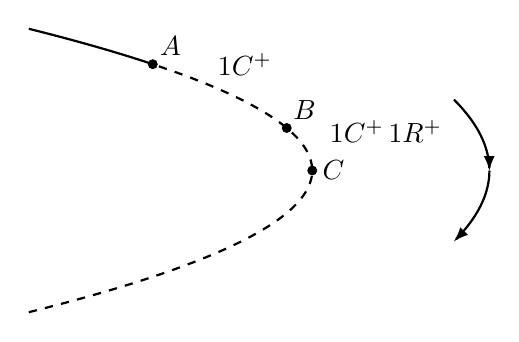
\begin{tikzpicture}[scale=0.9] \draw[thick, dashed]
    plot[smooth,domain=-2:1.5] ({-\x*\x},\x); \draw[thick]
    plot[smooth,domain=1.5:2] ({-\x*\x},\x);

    \draw[-latex, thick] plot[smooth,domain=1:0] ({2.5 + -0.5*\x*\x},\x);
    \draw[-latex, thick] plot[smooth,domain=0:-1] ({2.5 + -0.5*\x*\x},\x);

  \fill (-1.5^2,1.5) circle [radius=2pt];
  \fill (-0.6^2,0.6) circle [radius=2pt];
  \fill (0,0) circle [radius=2pt];

  \node at (-1.5^2 + 0.25,1.5 + 0.25) {$A$};
  \node at (-0.6^2 + 0.25,0.6 + 0.25) {$B$};
  \node at (0.3,0) {$C$};

  \node at (-1.5^2 + 1.3,1.6 - 0.1) {$1\mathbb{C}^{+}$};
  \node at (-0.6^2 + 1.4,0.6 - 0.05) {$1\mathbb{C}^+ \, 1\mathbb{R}^+$};
\end{tikzpicture}
\captionof{figure}{A schematic of the encountered eigenvalue crossing and the
  direction of the linear stability analysis in figure \ref{fig:lsa},
  $1\mathbb{C}^{+}$: conjugate pair of unstable eigenvalues, $1\mathbb{R}^+$ :
  real unstable eigenvalue}
\label{fig:schem_saddle}
\end{minipage}\hspace{10mm}
\begin{minipage}[b]{.35\textwidth}
  \centering
  \begin{tabular}{crrr}
  $n$ & $A$ ($H$) & $B$ ($P_3$) & $C$ ($SN$) \\
  \hline
  $64$ & $348.19$ & $353.356$ & $353.656$ \\
  $96$ & $348.19$ & $353.357$ & $353.654$ \\
  & & & \\
  & & & \\
\end{tabular}
\captionof{table}{Critical Reynolds numbers where crossings appear \newline \newline}
\label{tab:cross}
\end{minipage}
\end{minipage}
\smallskip

\begin{figure}[h]
  \centering
  \includegraphics[width=0.75\textwidth]{figs/lsa_sn96x96.pdf}
  \caption{Linear stability analysis around saddle-node (increasing and
    decreasing Reynolds number), the real part of the three largest eigenvalues
    are shown, grid $96 \times 96$} 
  \label{fig:lsa}
\end{figure}

Additionally, close to the saddle-node, another unstable branch emerges, which
was detected by starting the natural continuation algorithm near the critical
Reynolds of the fold. This branch is depicted in figure \ref{fig:branch2} and
contains unstable fixed points. The figure shows the projections onto the
$\Psi$ and $u_T$ planes to distinguish the branches. One can see that for the
new branch, the center value of the streamfunction is not changing
significantly, whereas, for both the asymmetric and the second branch, there is
a slight change in the horizontal velocity $u_T$. Further, this branch is
connected to point $B$, corresponding to another pitchfork, denoted by $P_3$.
Linear stability analysis around the pitchfork of this new branch (figure
\ref{fig:lsa_branch2}) reveals how the eigenvalues can be related to point $B$
(i.e. $P_3$).

\begin{figure}[h!]
  \centering
  \includegraphics[trim={0 0.8cm 0 0.5cm},clip,width=0.8\textwidth]{figs/branch2_64x64.pdf}
  \caption{3D plot of the asymmetric branch (blue) and second branch (light blue) and the
    connection of the two branches at pitchfork $P_3$ ($B$)}
  \label{fig:branch2}
\end{figure}

The emergence of the second branch provides an alternative perspective on the
problem. Since we are dealing with symmetric boundary conditions, we can
observe that the streamlines of the symmetric base solution in the four-sided
lid-driven cavity flow remains unchanged under a $\pi$-rotation and a
reflection on the diagonal combined with a change of sign (in terms of
streamfunction) of the cavity. The second symmetry is broken for the two
asymmetric branches, which only conserve the $\pi$-rotation symmetry. Figure
\ref{fig:sol_branch2} illustrates the two solutions of the additional pitchfork
emerging at $P_3$, and it can be seen that the rotational symmetry is no
longer valid for these branches. However, both branches exhibit the rotational
symmetry to one another.

\begin{figure}[h!]
\centering
\begin{subfigure}[b]{0.25\textwidth}
  \centering
  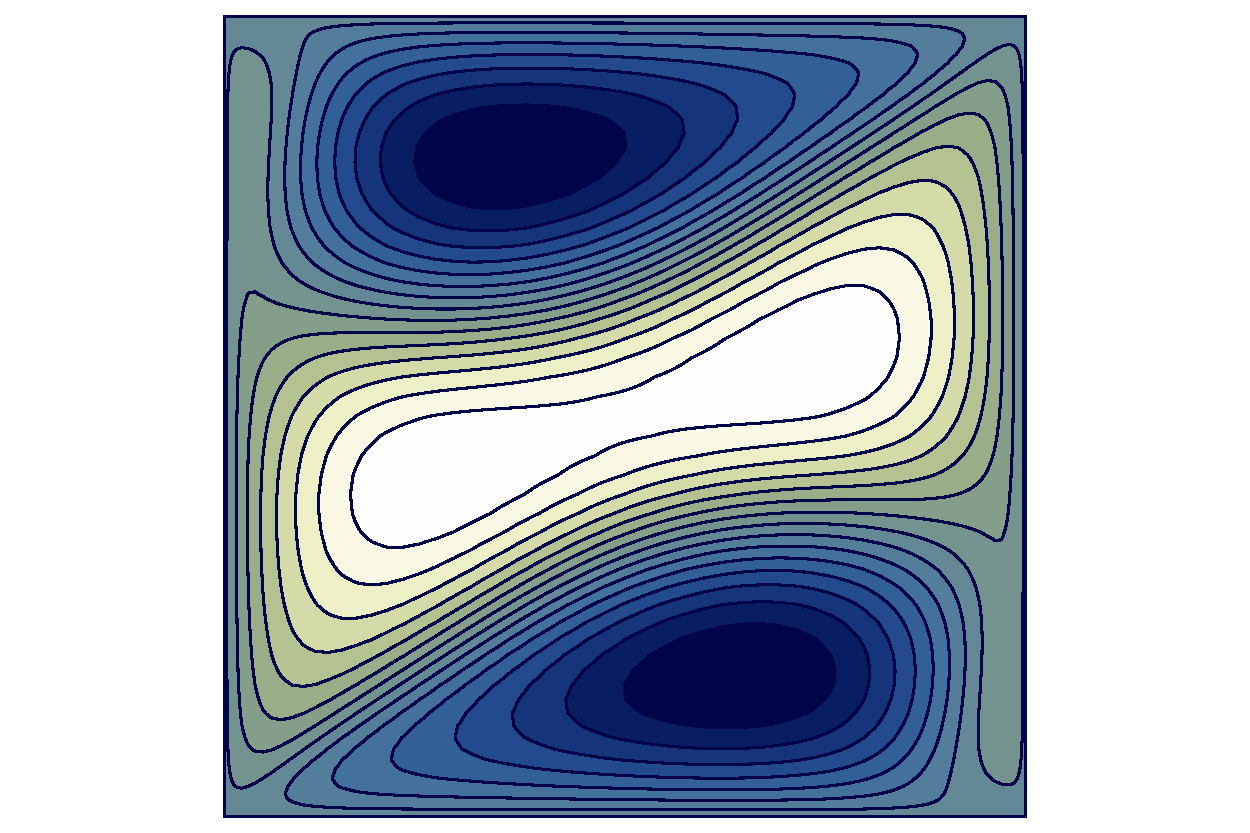
\includegraphics[trim={3.6cm 0 3.6cm 0},clip,width=\textwidth]{figs/psi_Re353.356_pf3.pdf}
  \caption{Pitchfork $P_3$}
\end{subfigure}
\begin{subfigure}[b]{0.25\textwidth}
  \centering
  \includegraphics[trim={3.6cm 0 3.6cm 0},clip,width=\textwidth]{figs/psi_Re375.000_branch2_u_t_smaller.pdf}
  \caption{Asymmetric solution 1}
\end{subfigure}
\begin{subfigure}[b]{0.25\textwidth}
  \centering
  \includegraphics[trim={3.6cm 0 3.6cm 0},clip,width=\textwidth]{figs/psi_Re375.000_branch2_u_t_bigger.pdf}
  \caption{Asymmetric solution 2}
\end{subfigure}
\caption{Streamlines of new branch, (a) $\pi$-rotation invariant, (b) and (c)
  are $\pi$-invariant with respect to each other}
\label{fig:sol_branch2}
\end{figure}

\begin{figure}[h!]
  \centering
  \includegraphics[trim={0 2.5cm 0 1cm},clip,width=0.8\textwidth]{figs/lsa_branch2_96x96.pdf}
  \caption{Linear stability analysis around connection $B$ of second branch
  (decreasing and then increasing Reynolds number), grid $96 \times 96$}
  \label{fig:lsa_branch2}
\end{figure}

The question that remains is what happens at the saddle-node at point $C$. The
schematic in figure \ref{fig:schem_saddle} shows the evolution of the
eigenvalues, and figure \ref{fig:lsa_zoom} shows a detail on the real part of
the eigenvalues for figure \ref{fig:lsa}. After the Hopf bifurcation ($A$), we
have a complex conjugate pair with nonzero imaginary components and a positive
real part. From pitchfork $P_3$ ($B$) onwards, the additional eigenvalue
$\lambda_3$ has a real part that also becomes positive. What occurs at the
saddle-node $C$ is, first of all, that the two eigenvalues lose their imaginary
part and become purely real. Moreover, this takes place at a nonzero real part.
What seems to be happening is that one of the complex pairs (now real) "jumps"
and becomes negative. The eigenvalue configuration is depicted in the complex
plane in figure \ref{fig:complexplane} to illustrate the behavior at the
saddle-node. The preceding explanation is speculative because we cannot be sure
that it is the eigenvalue corresponding to the complex pair that becomes
stable. It could be that two positive eigenvalues meet at the saddle-node.

Another reason for being cautious with our interpretation is that the
saddle-node is a highly degenerated point where the Jacobian is
ill-conditioned, therefore the accuracy of the steady flows, along the linear
stability analysis, may be at stake. Due to the degeneracy, it may even be that
the saddle-node corresponds to a double or triple zero, and multiple eigenvalue
crossings coincide. Nonetheless, these results were obtained on a large grid
for a pseudo-spectral code of size $96 \times 96$.

\begin{figure}[h!]
  \centering
  \includegraphics[width=0.7\textwidth]{figs/lsa_sn_zoom96x96.pdf}
  \caption{Zoom of figure \ref{fig:lsa} on saddle-node bifurcation, grid $96
    \times 96$} 
  \label{fig:lsa_zoom}
\end{figure}

\begin{figure}[!htbp]
\centering
\begin{subfigure}[b]{0.3\textwidth}
  \centering
  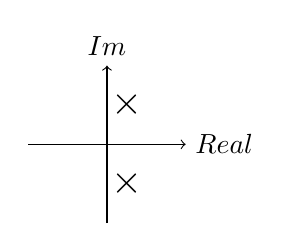
\begin{tikzpicture}
    \draw[->] (-1,0) -- (1,0) node[right] {$Real$};
    \draw[->] (0,-1) -- (0,1) node[above] {$Im$};
    \node at (0.25,0.5) {\textbf{\Large $\times$}};
    \node at (0.25,-0.5) {\textbf{\Large $\times$}};
  \end{tikzpicture}
  \caption{$1\mathbb{C}^+$, before saddle-node $C$ \newline}
\end{subfigure}
\begin{subfigure}[b]{0.3\textwidth}
  \centering
  \begin{tikzpicture}
    \draw[->] (-1,0) -- (1,0) node[right] {$Real$};
    \draw[->] (0,-1) -- (0,1) node[above] {$Im$};
    \node at (0.25,0) {\textbf{\Large $\times$}};
  \end{tikzpicture}
\caption{$2\mathbb{R}^+$, "just" before saddle-node $C$}
\end{subfigure}
\begin{subfigure}[b]{0.3\textwidth}
  \centering
  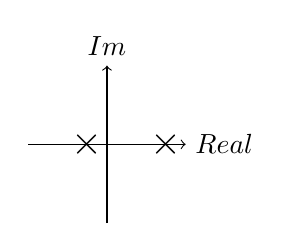
\begin{tikzpicture}
    \draw[->] (-1,0) -- (1,0) node[right] {$Real$};
    \draw[->] (0,-1) -- (0,1) node[above] {$Im$};
    \node at (0.75,0) {\textbf{\Large $\times$}};
    \node at (-0.25,0) {\textbf{\Large $\times$}};
  \end{tikzpicture}
\caption{$1\mathbb{R}^+$, at the saddle-node $C$ \newline}
\end{subfigure}
\caption{Visualization of the real and imaginary part of the complex conjugate pair
  $\lambda_1$ and $\lambda_2$ of figure \ref{fig:lsa} and \ref{fig:lsa_zoom}.}
\label{fig:complexplane}
\end{figure}
